% This is samplepaper.tex, a sample chapter demonstrating the
% LLNCS macro package for Springer Computer Science proceedings;
% Version 2.21 of 2022/01/12
%
% STUDENT TEMPLATE - Modified for local compilation
% Instructions:
% 1. Replace the title, author, and institute information below
% 2. Use your Student ID in \orcidID{...} (not ORCID)
% 3. For figures, use PDF format (preferred) or PNG/JPG
% 4. References are managed using BibTeX (references.bib file)
% 5. Compile with: pdflatex -> bibtex -> pdflatex -> pdflatex
%
\documentclass[runningheads]{llncs}
%
\usepackage[T1]{fontenc}
% T1 fonts will be used to generate the final print and online PDFs,
% so please use T1 fonts in your manuscript whenever possible.
% Other font encondings may result in incorrect characters.
%
\usepackage{graphicx}
% Used for displaying figures. For local compilation, use PDF, PNG, or JPG format.
% EPS files require Ghostscript (gs) to be installed.

\usepackage{float}
% For better control of figure placement
%
% Optional: Uncomment the following lines if you want clickable links
% and URLs in blue according to Springer's eBook style:
%\usepackage{color}
%\usepackage{hyperref}
%\renewcommand\UrlFont{\color{blue}\rmfamily}
%\urlstyle{rm}
%
\begin{document}
%
% ============================================================
% INSTITUTIONAL LOGOS - Add logos in upper left corner of title page
% ============================================================
% The logos are placed in the upper left corner of the title page.
% Adjust the height parameter (currently 0.9cm) to resize logos.
% Adjust \vspace*{-...} values to fine-tune vertical position.
% The spacing is adjusted to keep logos, title, and abstract on one page.
% ============================================================
\enlargethispage{3cm}
\vspace*{-2.0cm}
\noindent

\includegraphics[height=0.8cm]{NEU logo.png}\hspace{0.3cm}

\includegraphics[height=0.8cm]{FDA logo.png}
\vspace*{1.0cm}
% ============================================================

\title{Paper Title}
%
%\titlerunning{Abbreviated paper title}
% If the paper title is too long for the running head, you can set
% an abbreviated paper title here
%
% Replace with your information.
% NOTE: For students, use your Student ID instead of ORCID ID.
% Format: \orcidID{YourStudentID} (e.g., \orcidID{20201234})
% All authors belong to the same institution, so use \inst{1} for all.
\author{First Author\inst{1}\orcidID{20201234} \and
Second Author\inst{1}\orcidID{20205678} \and
Third Author\inst{1}\orcidID{20209012}}
% Example without Student ID (if not required):
% \author{Your Name\inst{1} \and
% Co-Author Name\inst{1}}
%
\authorrunning{F. Author et al.}
% First names are abbreviated in the running head.
% If there are more than two authors, 'et al.' is used.
%
\institute{Faculty of Data Science and Artificial Intelligence,\\
College of Technology, National Economics University\\
\email{your.email@neu.edu.vn}}
% If you have multiple authors from the same institution, use:
% \institute{Faculty of Data Science and Artificial Intelligence,\\
% College of Technology, National Economics University\\
% \email{author1@neu.edu.vn} \and
% \email{author2@neu.edu.vn}}
%
\maketitle              % typeset the header of the contribution
\vspace{-0.5cm}
\begin{abstract}
The abstract should briefly summarize the contents of the paper in
150--250 words.

\keywords{First keyword  \and Second keyword \and Another keyword.}
\end{abstract}
\vspace{-0.5cm}
% ============================================================
% STANDARD SCIENTIFIC PAPER STRUCTURE
% ============================================================
% The following sections follow the standard structure of a scientific paper.
% Replace the example content with your own research content.
% ============================================================
%
\section{Introduction}
% The introduction should:
% - Provide background and context for your research
% - State the problem or research question
% - Outline the objectives and contributions
% - Provide a brief overview of the paper structure

This section introduces the research topic, provides necessary background
information, and states the problem being addressed. The introduction should
clearly articulate the research objectives and the main contributions of the
paper. It typically ends with a brief outline of the paper structure.

Please note that the first paragraph of a section or subsection is
not indented. The first paragraph that follows a table, figure,
equation etc. does not need an indent, either.

Subsequent paragraphs, however, are indented.

\section{Related Work}
% The related work section should:
% - Review relevant previous research
% - Compare and contrast different approaches
% - Identify gaps in existing literature
% - Position your work within the existing body of knowledge

This section reviews relevant previous work in the field. It should
comprehensively survey existing approaches, methods, and findings related
to your research topic. The review should be organized thematically or
chronologically, and should clearly identify how your work differs from or
extends previous research.

\subsection{Previous Approaches}
% Use subsections to organize different aspects of related work

Previous research in this area has addressed various aspects of the problem.
For example, Author et al.~\cite{ref_article1} proposed a method that...

\subsection{Research Gaps}
% Identify what is missing in current research

Despite the progress made, several limitations remain in existing approaches...

\section{Methodology}
% The methodology section should:
% - Describe your approach, methods, or algorithms in detail
% - Explain the experimental setup
% - Provide sufficient detail for reproducibility
% - Include mathematical formulations if applicable

This section describes the methodology, approach, or algorithms used in your
research. It should provide sufficient detail for readers to understand and
potentially reproduce your work.

\subsection{Problem Formulation}
% Define the problem mathematically or conceptually

The problem can be formally stated as follows. Let $X$ represent...

\noindent Displayed equations are centered and set on a separate line.
\begin{equation}
x + y = z
\end{equation}

\subsection{Proposed Approach}
% Describe your method in detail

Our approach consists of the following steps:
\begin{enumerate}
\item First step description
\item Second step description
\item Third step description
\end{enumerate}

Figure~\ref{fig:method} illustrates the overall architecture and workflow of the proposed method.

\begin{figure}
\centering
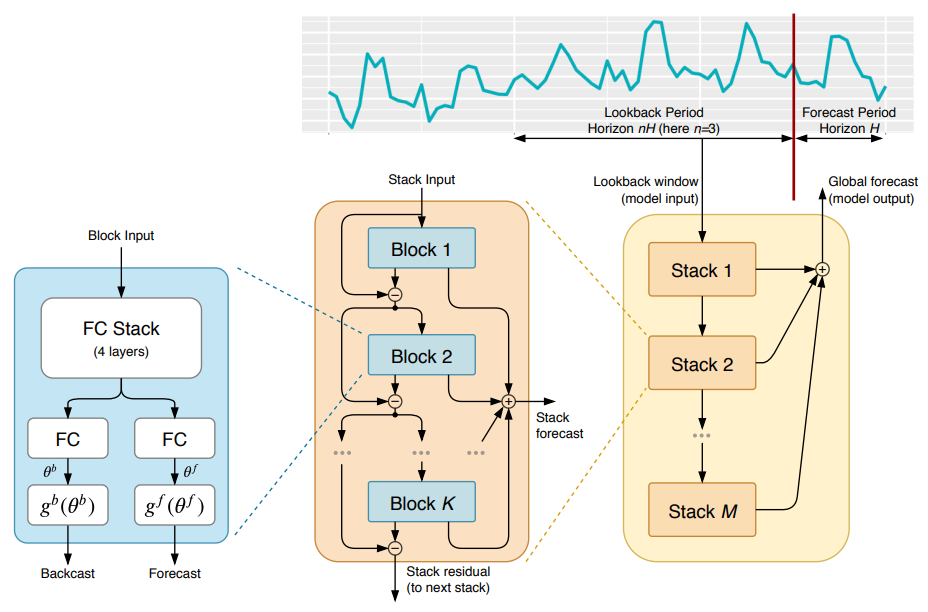
\includegraphics[width=\textwidth]{sample_method_fig.png}
\caption{Overview of the proposed method architecture and workflow.} \label{fig:method}
\end{figure}

\subsection{Algorithm Description}
% If you have algorithms, describe them here

The proposed algorithm can be summarized as follows:

\begin{theorem}
This is a sample theorem. The run-in heading is set in bold, while
the following text appears in italics. Definitions, lemmas,
propositions, and corollaries are styled the same way.
\end{theorem}
%
% the environments 'definition', 'lemma', 'proposition', 'corollary',
% 'remark', and 'example' are defined in the LLNCS documentclass as well.
%
\begin{proof}
Proofs, examples, and remarks have the initial word in italics,
while the following text appears in normal font.
\end{proof}

\section{Experiments and Results}
% The results section should:
% - Present experimental setup and datasets
% - Show experimental results (tables, figures, graphs)
% - Compare with baseline methods
% - Analyze and interpret the results

This section presents the experimental setup, datasets used, and the results
obtained. Results should be presented clearly using tables and figures, and
compared with baseline methods or previous approaches.

\subsection{Experimental Setup}
% Describe your experimental configuration

The experiments were conducted using the following setup:
\begin{itemize}
\item Hardware specifications
\item Software and libraries used
\item Parameter settings
\item Evaluation metrics
\end{itemize}

\subsection{Datasets}
% Describe the datasets used

We evaluated our approach on the following datasets...

\subsection{Results}
% Present your results with tables and figures

Table~\ref{tab1} presents a comparison of different methods.

\begin{table}
\caption{Comparison of different approaches.}\label{tab1}
\begin{tabular}{|l|l|l|}
\hline
Method & Metric 1 & Metric 2\\
\hline
Baseline & 0.XX & 0.XX\\
Method A & 0.XX & 0.XX\\
Proposed & 0.XX & 0.XX\\
\hline
\end{tabular}
\end{table}

% ============================================================
% FIGURE INSTRUCTIONS FOR STUDENTS:
% ============================================================
% To add a figure:
% 1. Place your figure file in the same directory as this .tex file
% 2. Uncomment ONE of the figure blocks below
% 3. Replace the filename with your actual figure filename
% 4. Add a reference in the text: (see Fig.~\ref{fig1})
% ============================================================

% Option 1: PDF figure (RECOMMENDED - works without Ghostscript)
% \begin{figure}
% \includegraphics[width=\textwidth]{results_figure.pdf}
% \caption{Performance comparison of different methods.} \label{fig1}
% \end{figure}

% Option 2: PNG/JPG figure (works without Ghostscript)
% \begin{figure}
% \includegraphics[width=\textwidth]{results_figure.png}
% \caption{Performance comparison of different methods.} \label{fig1}
% \end{figure}

% Option 3: EPS figure (requires Ghostscript installation)
% Only uncomment if you have Ghostscript (gs) installed:
% \begin{figure}
% 
\includegraphics[width=\textwidth]{fig1.eps}
% \caption{Performance comparison of different methods.} \label{fig1}
% \end{figure}

\subsection{Analysis}
% Analyze and interpret your results

The results demonstrate that our proposed method achieves...

\section{Discussion}
% The discussion section should:
% - Interpret the results in the context of the research question
% - Discuss limitations and potential issues
% - Compare findings with related work
% - Explain unexpected results

This section discusses the implications of the results, their significance,
and how they relate to the research objectives stated in the introduction.
It should also address limitations of the work and potential areas for
improvement.

\section{Conclusion}
% The conclusion should:
% - Summarize the main contributions
% - Restate the key findings
% - Suggest future work directions

This section summarizes the main contributions of the paper, restates the
key findings, and suggests directions for future research. It should be
concise and avoid introducing new information.

For citations of references, we prefer the use of square brackets
and consecutive numbers. Citations are managed using BibTeX.
Example citations: journal articles~\cite{ref_article1}, an LNCS 
chapter~\cite{ref_lncs1}, a book~\cite{ref_book1}, proceedings 
without editors~\cite{ref_proc1}, and a homepage~\cite{ref_url1}. 
Multiple citations are grouped
\cite{ref_article1,ref_lncs1,ref_book1},
\cite{ref_article1,ref_book1,ref_proc1,ref_url1}.

% ============================================================
% Author Contributions Section
% ============================================================
% This section describes the individual contributions of each author.
% Use the CRediT (Contributor Roles Taxonomy) format or describe
% contributions in your own words.
% ============================================================

\begin{credits}
\subsubsection{Author Contributions}
% Describe each author's specific contributions to the work.
% Example format using CRediT taxonomy:
% - Conceptualization: idea, hypothesis
% - Methodology: design of methodology
% - Software: programming, software development
% - Validation: verification, replication
% - Formal analysis: statistical analysis, mathematical analysis
% - Investigation: conducting experiments, data collection
% - Resources: provision of materials, computing resources
% - Data curation: data management, organization
% - Writing - original draft: initial writing
% - Writing - review \& editing: revision, editing
% - Visualization: figures, diagrams
% - Supervision: oversight, leadership
% - Project administration: coordination, management
% - Funding acquisition: securing funding

\textbf{First Author:} Conceptualization, Methodology, Software, Writing - original draft, Visualization.

\textbf{Second Author:} Methodology, Formal analysis, Investigation, Data curation, Writing - review \& editing.

\textbf{Third Author:} Validation, Resources, Writing - review \& editing, Supervision.

% Alternative format (descriptive):
% First Author contributed to the conceptualization of the research idea,
% developed the methodology, implemented the software, created visualizations,
% and wrote the initial draft. Second Author conducted the formal analysis,
% performed the experimental investigation, curated the datasets, and
% contributed to writing and editing. Third Author validated the results,
% provided computational resources, supervised the project, and reviewed
% and edited the manuscript.

\end{credits}
%
% ---- Bibliography ----
%
% BibTeX is used for managing references.
% 1. Create a .bib file (e.g., references.bib) with your references
% 2. Use the bibliography style 'splncs04' for LNCS format
% 3. Compile with: pdflatex -> bibtex -> pdflatex -> pdflatex
%
\bibliographystyle{splncs04}
\bibliography{references}
%
% If you prefer manual bibliography (not recommended), uncomment below:
% \begin{thebibliography}{8}
% \bibitem{ref_article1}
% Author, F.: Article title. Journal \textbf{2}(5), 99--110 (2016)
% \end{thebibliography}
\end{document}
